\documentclass[conference]{style/IEEEtran}
\IEEEoverridecommandlockouts
\usepackage{multirow}
\usepackage{amsmath,amssymb,amsfonts}
\usepackage{algorithmic}
\usepackage{graphicx}
\usepackage{textcomp}
\usepackage{xcolor}
\def\BibTeX{{\rm B\kern-.05em{\sc i\kern-.025em b}\kern-.08em
    T\kern-.1667em\lower.7ex\hbox{E}\kern-.125emX}}
\usepackage[style=ieee, backend=biber, sorting=none]{biblatex}
\addbibresource{references/references.bib}
    
\begin{document}

\title{A Natural Language Processing Approach for the Digitalization of Roaming Agreement}

%\author{\IEEEauthorblockN{1\textsuperscript{st} Given Name Surname}
%\IEEEauthorblockA{\textit{dept. name of organization (of Aff.)} \\
%\textit{name of organization (of Aff.)}\\
%City, Country \\
%email address or ORCID}
%\and
%\IEEEauthorblockN{2\textsuperscript{nd} Given Name Surname}
%\IEEEauthorblockA{\textit{dept. name of organization (of Aff.)} \\
%\textit{name of organization (of Aff.)}\\
%City, Country \\
%email address or ORCID}
%\and
%\IEEEauthorblockN{3\textsuperscript{rd} Given Name Surname}
%\IEEEauthorblockA{\textit{dept. name of organization (of Aff.)} \\
%\textit{name of organization (of Aff.)}\\
%City, Country \\
%email address or ORCID}
%\and
%\IEEEauthorblockN{4\textsuperscript{th} Given Name Surname}
%\IEEEauthorblockA{\textit{dept. name of organization (of Aff.)} \\
%\textit{name of organization (of Aff.)}\\
%City, Country \\
%email address or ORCID}
%}

\maketitle

\begin{abstract}
Roaming is the capability of a subscriber to have persistence of service in a visited mobile network managed by a different operator. To achieve this persistence of connectivity, it is necessary for operators to agree on technical, commercial and legal aspects in what is known as a Roaming Agreement. Currently, Roaming Agreement negotiation uses asynchronous flow such as email or even regular mail. The main phase in building the roaming agreement is known as the drafting phase, which is a time-consuming process with limited assurance and transparency on handling the drafting events. To address the lack of transparency and reduce the drafting time, this paper proposes a framework that automates the process of drafting and negotiation of the roaming agreement and enables better accessibility. The proposed framework exploits a Natural Language Processing (NLP) engine as a starting point for the digitalization of the negotiation process towards transparent drafting of Roaming Agreements. Extensive experiments on real roaming agreements show the superiority of our proposed framework in drafting the roaming agreements against the traditional drafting and negotiation process with prediction accuracy over 80.0\%.
\end{abstract}

\begin{IEEEkeywords}
Roaming Agreement, Natural Language Processing, Telecommunication
\end{IEEEkeywords}

\section{Introduction}
The roaming service maintains the persistent connectivity of subscribers in different networks and locations. Roaming describes the capability of a subscriber to access mobile services offered by the visited public mobile network (VPMN) through the home public mobile network (HPMN), when roaming outside the coverage range of the HPMN \cite{Tanaka2013}. However, before ensuring persistent connectivity in VPMN the Mobile Network Operators (MNOs) must reach an agreement regarding the technical, commercial and legal relationships known as the Roaming Agreement (RA). In this regard, it is possible to establish three stages within the RA: \textit{drafting}, \textit{testing} and \textit{implementation}. The testing and implementation phases are straight forward as they are related with implementing what is agreed on the drafting phase. However, the drafting phase is ambiguous and involves multiple iterations of exchange of draft text and proposed articles between both parties, i.e. the MNOs. 

Therefore, in order to reduce the exerted efforts and standardize the technical, commercial and legal aspects of the RA, the GSM Association broadly outlines the content of such RA in standardized form for its members \cite{Ferwerda2018}. 
In addition, many organizations attempt to unify RAs. For example, Rocco\footnote{Rocco Group: https://www.rocco.group}, which is a company specialized in telecommunication reports including roaming agreements, provides a list of the most commonly used GSMA standards. It summarizes these standards as follows \cite{ROCCO2017}: (1) AA.12 constitutes the permanent reference document; (2) AA.13 contains the common annexes with operational information (e.g., information on tap file, billing data, settlement procedure, customer care, fraud, etc.) and (3) AA.14 involves the individual annexes containing information about the operator (e.g., contact details of the roaming team, fraud team, IREG team, TADIG team, etc.).

While it is true that it is not mandatory to follow the standards proposed by the GSMA organization, according to authoritative voices in the field of negotiating RA drafting, most MNOs follow them strictly \cite{ROCCO2017a}. Therefore, the first point to consider in the RA drafting is how far it is deviated from the GSMA's proposed standards. Thus, during the drafting process of the agreement, the parties should analyze the sub-articles contained in the GSMA standard templates. This necessitates discretizing the bulk of the roaming agreement template and classifying each word/clause from an existing classes as follows:

\begin{enumerate}
\item Specify the value of certain \textit{variables} that are found in a certain text, such as dates, names of MNOs, locations and others.
\item Introduce certain \textit{variations} in the articles/sub-articles, usually identified as part of the text with different paraphrasing.
\item Leave an article/sub-article as found in the template (RA draft); thereby establishing a \textit{standard clause}.
\item Introduce completely new articles/sub-articles that respond to particular interests by constituting \textit{customized texts}.
\end{enumerate}

However, the \textit{drafting} of a RA goes through a complex negotiation process in which, at present, the parties still use asynchronous flows such as e-mail or even regular mail to exchange the information. Thus, this traditional negotiation process has multiple drawbacks including lacks of transparency, which can lead to violations of the RA by MNOs. In addition, this process is laborious and time consuming. As experts point out, the entire process can take up to one month, depending on the responsiveness of the MNOs \cite{ROCCO2017a}. Therefore, it is necessary to provide a transparent digitalization system for RA drafting negotiations, which guarantees transparency and shortening the negotiation time, which guarantees transparency and shortening the negotiation time, which could be in days or even weeks. Hence, this work develops a framework that exploits the advancement in the Natural Language Processing (NLP) discipline and use it as a legal text in the digitalization engine. This NLP Engine constitutes the starting point for the digitalization of the negotiation process towards a transparent drafting of Roaming Agreements. The proposed NLP Engine analyzes articles and sub-articles of the RA by determining the existence of variables, variations, standard clauses and customized texts. To do so, the proposed NLP Engine relies on the advancement of NLP techniques such as Named Entity Recognition (NER) and Part of Speech (POS) in drafting RAs.

% using the unstructured data information discovery tool \textit{Amazon Comprehend} and, on the other hand, by establishing an comprehensive comparison between texts based on \textit{similarity} determination techniques. The procedures for integrating tools, NLP techniques, pre-processing and post-processing constitute a methodological framework designed for the use case and included within an unstructured text processing tool. This article includes not only the design phase, but also the implementation and evaluation of the NLP Engine tool.

% The rest of this manuscript is structured as follows: Section 2 presents the related work in order to determine the novelty of the proposed topic. Section 3 establishes the designed methodology. The implementation of our system are described in Section 4. Section 5 discusses the results of conducted experiments. Finally, the conclusions of the manuscript are included in Section 6.
\section{Related work}\label{related}

The existing work that is related to the RAs can be categorized into two main categories. The first category encompasses the work, which focused on transparent digitalization of RAs~\cite{9369516, 9024541, Huillet2020}, whereas the second category includes the works that apply existing NLP techniques-based text processing systems~\cite{8487847, 9138070, 9104105}.

Both in the scientific literature and business environments, there are important approaches to RA digitalization. Thus, the work discussed in~\cite{9369516} proposes a dynamic RA between the Local 5G Operator and the MNO. The interaction between the two entities takes place through an Ethereum based platform. Despite the contributions of this work in the RA \textit{implementation} phase, the fact of performing the implementation on the Ethereum network implies that the participating MNOs will bear the high cost of gas fees for the transactions. Additionally, although the authors justify the latency given that they repeated the experiment 100 times, the proof of work nature of the network implies drafting actions are likely to suffer congestion anytime. A second approach focuses uniquely on the billing of the services obtained as a result of the RA is reported in~\cite{9024541}. This agreement is incorporated as part of a chaincode of a Hyperledger Fabric Blockchain (HFB) network so the work contributes significantly to the digitalization process of the RA, allowing for a faster, more seamless process in which payments can be requested and obtained quickly due to less need for manual intervention. Although this work also constitutes an important contribution regarding the use of HFB in the field of telecommunications to address problems around Managing RAs, Inter-carrier Settlements, and Mobile Number Portability, its approach is one of review and proposal, however, it lacks an implementation section that would allow demonstrating the feasibility of the proposals. The contextualization of this system in the business environment is proposed by important MNOs such as Telefonica, Deutsche Telekom, and Vodafone which use blockchain for Roaming settlement within the framework of the RA between the parties~\cite{Huillet2020}. This proposal is also of considerable value in the business environment, however, its focus relates only to the \textit{implementation} phase of the RA and not to the \textit{drafting} phase. 

Additionally, the scientific literature addresses text processing systems based on NLP techniques in domains such as the judiciary. Thus, the approach introduced in~\cite{8487847} addresses the process of digitalization in the judicial sectors from archives of judicial records for which the authors have designed a text analysis tool that includes grammatical analysis of documents in English based on NLP techniques. The proposed article also constitutes an important contribution in terms of the design of the linguistic analysis based on NLP techniques. However, it lacks formal evaluation in terms of accuracy of NLP implementation. In addition, the work reported in~\cite{9138070} applies NLP-based processing techniques for information retrieval from spreadsheets and describes technologies for storing and retrieving database information. NLP techniques such as sentence tokenization, word tokenization, removing stopwords and lemmatization are part of the parsing stage of the work. The work constitutes a valuable contribution in terms of design and implementation of the tool, however, it lacks demonstration of the feasibility of use, as well as determination of the accuracy of the NLP techniques applied. Finally, authors of~\cite{9104105} propose a model for implementing sentimental analysis using Amazon Comprehend. This system performs an audio-to-text transcription and then performs the processing of the obtained text. Although the value of the contribution lies in the use of NLP techniques from the Amazon Comprehend tool, the paper lacks a formal results section, therefore it is difficult to determine the accuracy of the proposed tool. 

Although these studies constitute a relevant part of related work, e.g., by integrating useful tools such as Amazon Comprehend or detailing the use of techniques such as tokenization, the scientific literature does not address scenarios for the telecommunication field and even less in the context of a transparent digitalization of the RA. Therefore, and to the best of our knowledge, we can affirm that our work introduces a topic with a high degree of novelty.
\section{NLP Engine methodology}\label{methodology}
In general, our design consists of the following two approaches (which we discuss in more detail in this section): \textit{detection} and \textit{comparison}. While \textit{detection} has symbols as basic processing unit, \textit{comparison} has sub-articles as basic processing unit. \textit{Detection} represents the capability to detect \textit{variables} in a text file, i.e., the RA. For this purpose, \textit{Amazon Comprehend} constitutes the enabling technology of the \textit{detection} approach, since it is a service that uses NLP techniques to extract insights about the content of text documents by recognizing  the  entities,  key  phrases,  language,  sentiments,  and  other  common  elements  in  a  text \cite{AWS2021}.

\textit{Comparison} represents the capability to find \textit{similarities} and differences between the sub-articles present in the RA concerning the sub-articles present in the GSMA standard template. In this regard, \textit{text similarity} constitutes the enabling technology of the \textit{comparison} approach, since it is a resource commonly used for pattern classification, clustering, and information retrieval problems \cite{7429408}. We employ \textit{Jaccard's similarity} which is defined as the size of the intersection divided by the size of the union of two sets \cite{Gupta2018}. As a result of the \textit{comparison}, it is determined that while an almost total coincidence between texts at the sub-article level represents a \textit{standard clause}, an almost null coincidence between texts (or simply the non-existence of a sub-article of the GSMA standard template in the RA) represents a \textit{customized text}. Thus, the intermediate case is represented by the \textit{variation} in which there is a high coincidence between sub-articles, and the existing differences are given by the presence of \textit{variables} such as the commercial names of MNOs and the start date of the RA. The next section integrates tools, NLP techniques, and text processing techniques as part of the designed methodology.

\subsection{Designed Methodology}
The flow chart in Fig.~\ref{fig1} is a general scheme of the methodology designed for the NLP Engine, which will be explained in detail below.

\begin{figure}[htbp]
\centerline{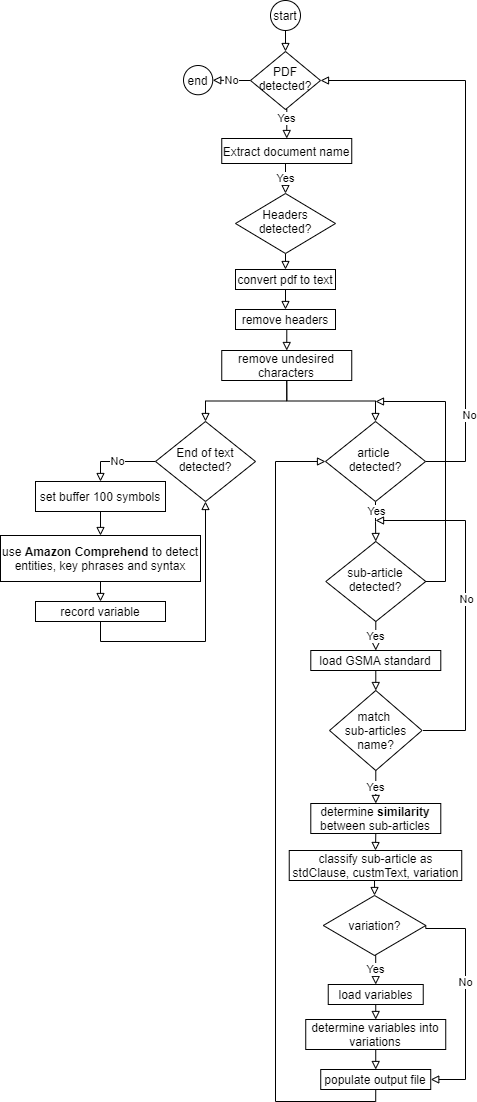
\includegraphics[width=0.4\textwidth]{images/methodology.png}}
\caption{Overview of the designed methodology.}
\label{fig1}
\end{figure}

The starting point of the methodology is the decompression and content extraction of PDF files (each PDF file contains a RA). The file name is used as one of the identifiers of the output file. The next step is to find similarities in document texts so that headers and footers are detected to avoid undesired characters. For that purpose, the mechanism used is the detection of different font sizes and weights. Once the PDF format has been converted to text, headers, and footers as well as undesired characters are removed. It is now possible to perform both \textit{detection} and \textit{comparison}.

The \textit{detection} phase includes a requirement associated with the Amazon Comprehend tool regarding the number of symbols to be sent via REST API. For this reason, the text is segmented into pieces of 100 symbols. For each symbol chunk the API outputs entities, key phrases and sentiment in JavaScript Object Notation (JSON) format \cite{AWS2021}, which must be grouped and further processed. The designed logic collects the most important fields such as: 'BeginOffset', 'EndOffset', 'Score', 'Text', 'Type', 'PartOfSpeech', and 'Tag'. In turn, it adds to these the 'Frequency' field that stores the number of repetitions of the entity stored in the 'Text' field. Once this filtering has been done, entities are sorted according to a logic that defines their relevance degree. The designed logic is particularized according to the type of \textit{variable} to be detected. For instance, for the name of the MNO, the 'Score', 'Frequency', and 'BeginOffset' are prioritized, in addition to verifying the number of occurrences within the key phrases. The detected \textit{variables} are stored to be used later to determine which ones are part of the \textit{variations} or \textit{customized texts}.

The \textit{comparison} phase implies to separate by articles and then by sub-articles. Since several of the possibilities of article names are loading in the NLP Engine is easy to locate the corresponding article in the GSMA standard template and therefore, to establish comparisons at the sub-article level. \textit{Jaccard's similarity} associates a score to the sub-article ID. Thus, a sub-article is considered a \textit{standard clause} whether the score assigned is greater than 0.85 (score $\geq$ 0.85). In addition, a sub-article is considered a \textit{custom text} whether the score assigned is less than 0.15 (score $\leq$ 0.15). Finally, a sub-article is considered a \textit{variation} whether the score assigned is between 0.85 and 0.15 (0.15 $<$ score $<$ 0.85). At this point, the NLP Engine is ready to populate the output file, inspecting in case of to have tagged the sub-articles as \textit{variation} or \textit{customized texts}, the \textit{variables} that it contains.
\input{sections/SystemImplementation}
\section{Discussion of Results}\label{results}
Our NLP Engine architecture receives PDF files as inputs, and PDF files normally consist of unstructured text. Because of this, undesired characters may remain despite text parsing. Therefore, it is mandatory to determine the \textit{accuracy} of the results obtained once the output JSON file has been populated. For this purpose, two types of experiments have been conducted to determine the \textit{accuracy} of the results. On the one hand, a simple inspection at the sub-article level and on the other hand, a verification based on symbol comparison. The tests were performed on two RA samples of the MNOs Proximus and Orange \cite{proximus}. Each experiment is described below and the results obtained are discussed in the same section.

\subsection{Accuracy determination based on a simple inspection at sub-article level}
The first accuracy analysis consists of visually determining, i.e., human-eye inspection, whether each sub-article of the RA constitutes a \textit{variation}, a \textit{standard clause} or a \textit{customized text} concerning the GSMA standard template. The results obtained are then compared with the values populated in the NLP Engine output file, for the same sub-article. Considering that the results obtained from the simple inspection constitute the observations and the values collected from the sub-articles classification file constitute the predicted values, the following confusion matrices allow us to analyze the results for each sample RA. In this regard, the confusion matrix in Table~\ref{table1} indicates that the \textit{accuracy} at which the 72 sub-articles analyzed are satisfactorily classified by the NLP Engine as \textit{standard clauses}, \textit{variations} or \textit{customized texts} is acceptable. Proof of this is the fact that the main diagonal of the matrix contains the highest number of True Positives. Table~\ref{table3} summarizes the accuracy of the NLP Engine's sub-article classification capability in percentage terms as \textit{standard clauses}, \textit{variations} and \textit{customized texts}.

\begin{table}[htbp]
\caption{Confusion Matrix for Proximus Roaming Agreement.}
\begin{center}
\begin{tabular}{|c|c|c|c|}
\hline
\textbf{n = 72} & \textbf{\textit{stdClause}}& \textbf{\textit{variation}}& \textbf{\textit{customText}} \\
\hline
\textbf{\textit{stdClause}}& 21 & 3 & 1 \\
\hline
\textbf{\textit{variation}}& 2 & 35 & 4 \\
\hline
\textbf{\textit{customText}}& 0 & 1 & 5 \\
\hline
\end{tabular}
\label{table1}
\end{center}
\end{table}

\begin{table}[htbp]
\caption{Confusion Matrix for Orange Roaming Agreement.}
\begin{center}
\begin{tabular}{|c|c|c|c|}
\hline
\textbf{n = 86} & \textbf{\textit{stdClause}}& \textbf{\textit{variation}}& \textbf{\textit{customText}} \\
\hline
\textbf{\textit{stdClause}}& 14 & 0 & 1 \\
\hline
\textbf{\textit{variation}}& 1 & 8 & 0 \\
\hline
\textbf{\textit{customText}}& 4 & 1 & 57 \\
\hline
\end{tabular}
\label{table2}
\end{center}
\end{table}

Table ~\ref{table2} shows satisfactory results for the NLP Engine's predictive capability, i.e., regarding the \textit{accuracy} at which the NLP Engine correctly classifies the sub-articles as \textit{standard clauses}, \textit{variations}, or \textit{customized texts} for the Orange sample RA. Using the same evaluation criteria, it is observed how the main diagonal of the confusion matrix in Table~\ref{table2} has the highest number of True Positive. Table~\ref{table3} also summarizes the accuracy of the NLP Engine's sub-article classification capability in percentage terms as \textit{standard clauses}, \textit{variations} and \textit{customized texts}.

\begin{table}[htbp]
\caption{Summary of accuracy determination for simple inspection at sub-article level.}
\begin{center}
\begin{tabular}{|c|c|c|c|}
\hline
\textbf{} & \textbf{\textit{Proximus}}& \textbf{\textit{Orange}} \\
\hline
\textbf{\textit{stdClause}}& 80.9\% & 92.9\% \\
\hline
\textbf{\textit{variation}}& 82.9\% & 87.5\% \\
\hline
\textbf{\textit{customText}}& 80.0\% & 91.2\% \\
\hline
\end{tabular}
\label{table3}
\end{center}
\end{table}

Beyond the fact that the results themselves can be considered as acceptable, the other behavior to be highlighted in Table~\ref{table3} is the greater classification capacity into \textit{standard clauses}, \textit{variations} and \textit{customized texts} of the NLP Engine in one document concerning another.

\subsection{Accuracy determination based on symbol comparison}
The second accuracy analysis involves establishing a comparison between the sub-articles populated in the output file concerning the sub-articles existing in the input file containing the RAs. This comparison is performed at the symbol level, considering the order of appearance of each symbol. For that purpose, the text comparison tool Countwordsfree (\cite{countwordsfree}) is used by manually copying sub-article by sub-article. For each sub-article, the following values are determined:

\begin{enumerate}
\item Common percentage of symbols between compared sub-articles.
\item Difference percentage of symbols between compared sub-articles.
\item Common symbols between compared sub-articles.
\item Difference symbols between compared sub-articles.
\end{enumerate}

\begin{figure}[htbp]
\centerline{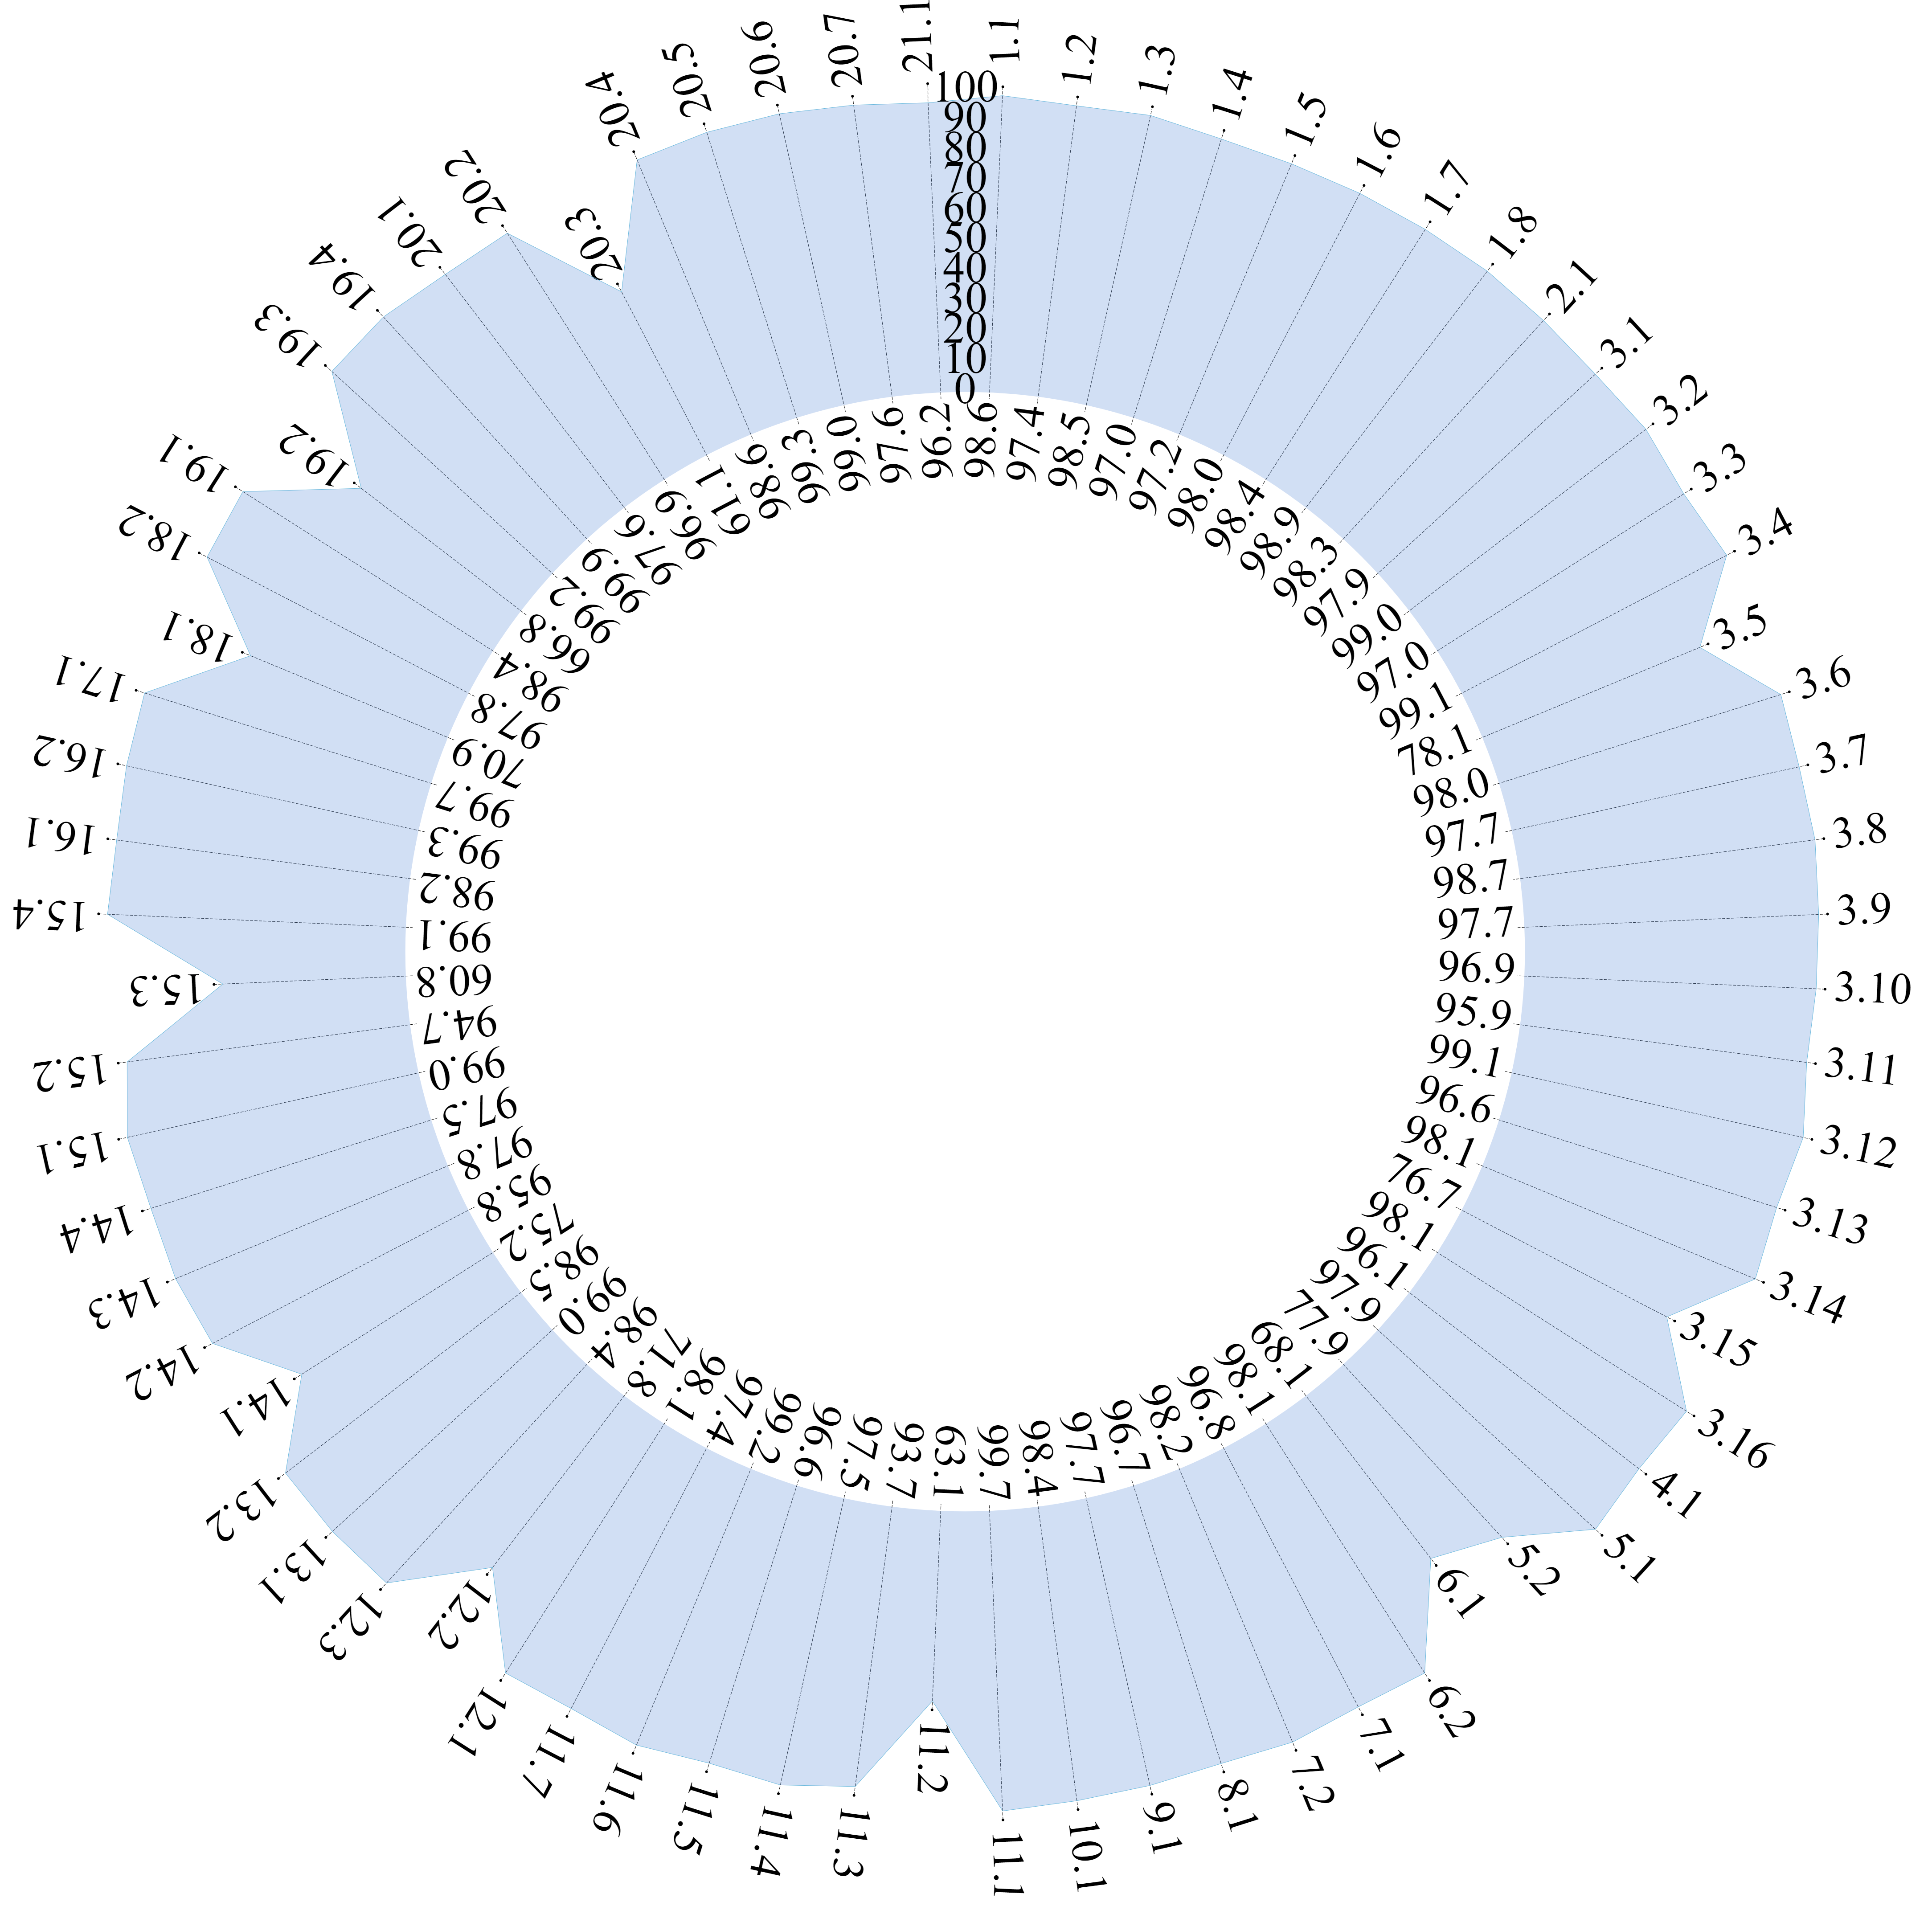
\includegraphics[width=0.43\textwidth]{images/Proximus.png}}
\caption{Common percentage of symbols for Proximus Roaming Agreement.}
\label{fig3}
\end{figure}

\begin{figure}[htbp]
\centerline{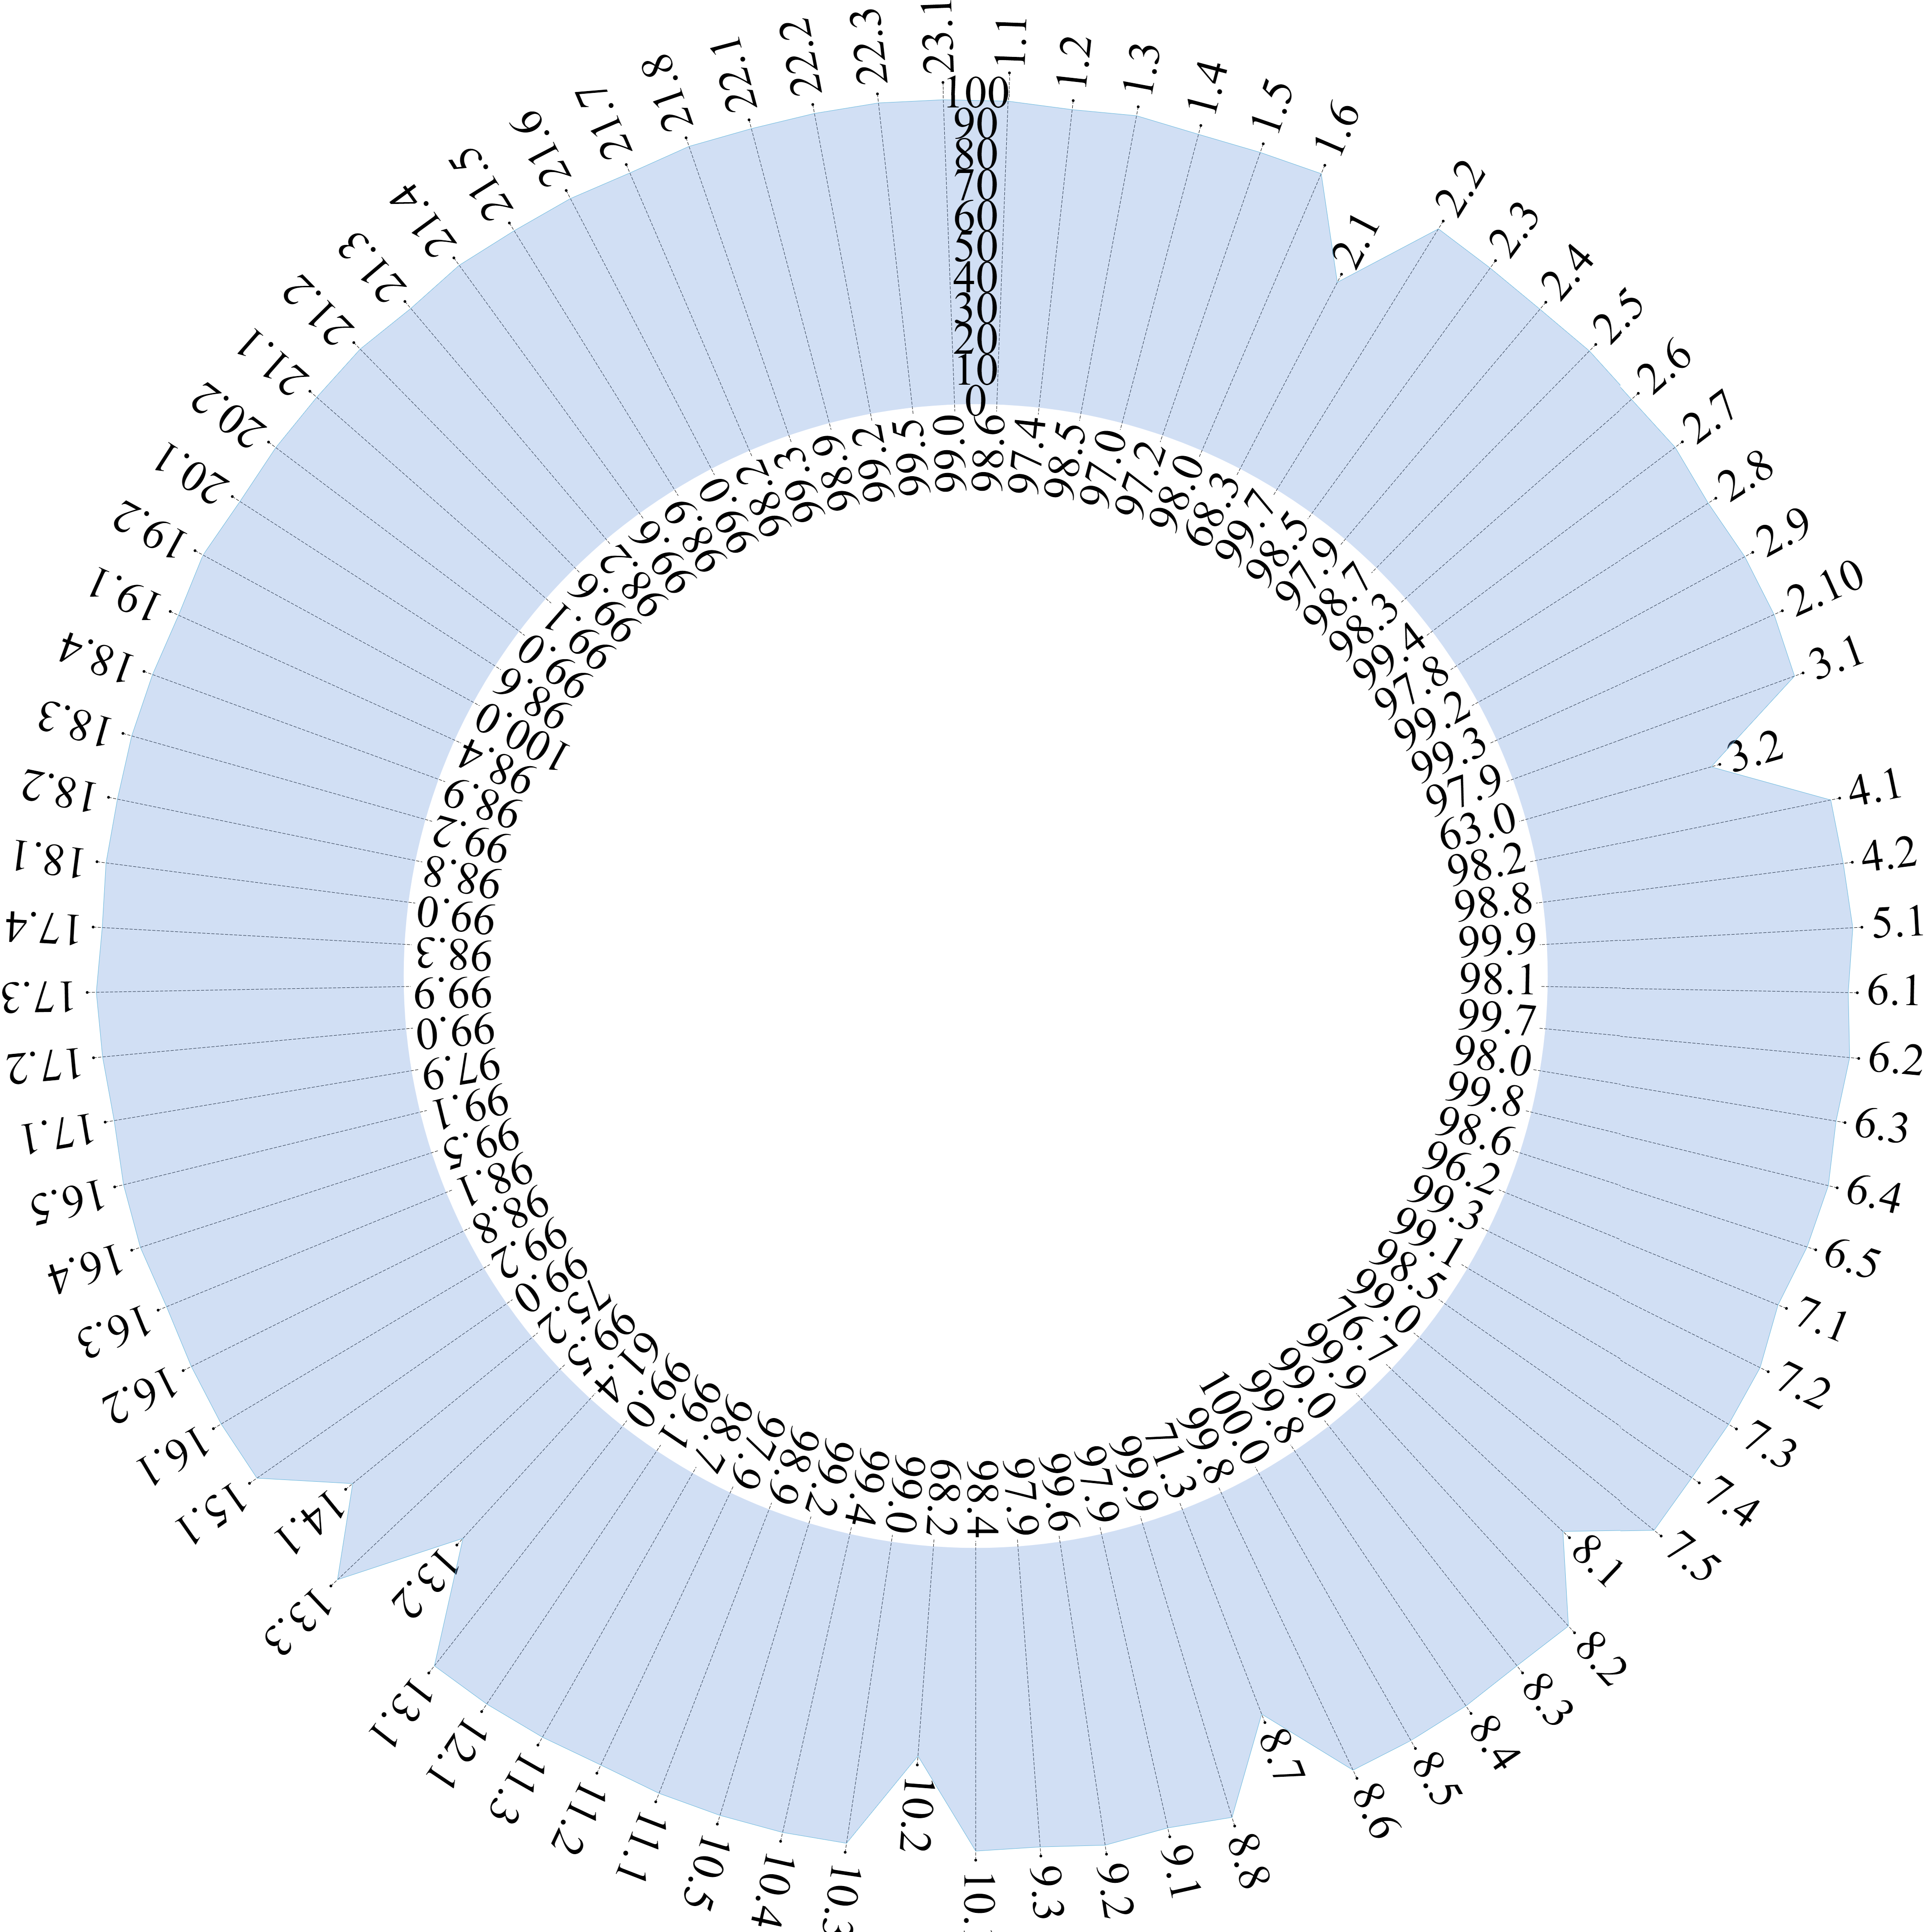
\includegraphics[width=0.43\textwidth]{images/Orange.png}}
\caption{NLP Engine overall architecture for Orange Roaming Agreement.}
\label{fig4}
\end{figure}

The illustrated radar charts allow us to analyze the results for each RA. The radar chart contains in the inner radius the common percentage of symbols between compared sub-articles and in the outer radius the identifier of the compared sub-article. Fig.~\ref{fig3} shows a comparison in terms of the common percentage of symbols between compared sub-articles for the Proximus sample RA. The conclusion that can be reached by simple inspection is that only 11 of the 72, i.e.,  84.7\% of the analyzed sub-articles are affected, mostly by the introduction of undesired characters when the output file was populated.

Similarly, Fig.~\ref{fig4} shows a comparison in terms of the common percentage of symbols between the sub-articles compared for the Orange sample RA. In this case, only 7 of the 86, i.e., 91.9\% of the analyzed sub-articles are affected by the introduction of undesired characters when the output file is populated, thus improving the results obtained for the Proximus sample RA.

%\subsection{Analysis of the novelty of the contribution}

%\begin{table}[htbp]
%\caption{Analysis of the novelty of the contribution.}
%\begin{center}
%\begin{tabular}{|c|c|c|c|c|c|c|c|}
%\hline
%\multirow{2}{*}{\textbf{Field}} & %\multirow{2}{*}{\textbf{C}} & %\multicolumn{3}{c|}{\textbf{RA phase}} & %\multicolumn{3}{c|}{\textbf{NLP  Engine}} \\ %\cline{3-8} 
%&  & Dr & I & T & D & I & T \\ \hline
%\textbf{} & our contribution &  &  &  &  & &  \\ %\hline
%\multirow{3}{*}{\textbf{RA}} 
%& \cite{9369516} &  &  &  &  &  &  \\ \cline{2-8} 
%& \cite{9024541} &  &  &  &  &  &  \\ \cline{2-8} 
%& \cite{Huillet2020} &  &  &  &  &  &  \\ \hline
%\multirow{3}{*}{\textbf{NLP}} 
%& \cite{8487847} &  &  &  &  &  &  \\ \cline{2-8} 
%& \cite{9138070} &  &  &  &  &  &  \\ \cline{2-8} 
%& \cite{9104105} &  &  &  &  &  &  \\ \hline
%\end{tabular}
%\label{table3}
%\end{center}
%\end{table}

\section{Conclusions}
The designed NLP-based methodology digitizes the roaming agreement by classifying the sub-articles of the roaming agreement as \textit{standard clauses}, \textit{variations} and \textit{customized texts}. The test phase allows to evaluate the results obtained from two types of experiments conducted to measure the accuracy to establish that on the one hand, the accuracy  determination  based  on  a  simple  inspection  at sub-article level determines for the first sample roaming agreement, an accuracy of 80.9\% in the classification of \textit{standard clauses}, an accuracy of 82.9\% in the classification of \textit{variations} and an accuracy of 80\% in the classification of \textit{customized texts}. These results are improved for the second sample roaming agreement with an accuracy of 92.9\% in the classification of \textit{standard clauses}, an accuracy of 87.5\% in the classification of \textit{variations} and an accuracy of 91.2\% in the classification of \textit{custom texts}. On the other hand, the determination of the accuracy based on the comparison of symbols determines for the first roaming agreement sample, an accuracy of 84.7\% of the total of 72 analyzed sub-articles with a common percentage of favorable symbols. This result is also improved for the second roaming agreement sample with an accuracy of 91.9\% of the total of 86 sub-articles analyzed with a common percentage of favorable symbols. Therefore, the results demonstrate the feasibility of applying the proposed methodology. As part of a process of continuous improvement of the designed methodology within future research lines we aim to conduct other accuracy tests applying other similarity classes, e.g., cosine similarity in order to improve the results obtained.

The proposed NLP Engine constitutes a part of a project that has as main objective of transforming the current Telecommunication Roaming Agreement drafting and negotiation process into a digitalized version based on the transparency promoted by blockchain technology, future research works include the design, development and evaluation of the rest of the sub-systems that mainly include the smart contracts that automate the negotiation process, as well as the integration with the developed NLP Engine.

%\section{Acknowledgment}\label{acknowledgment}
This research was funded by Linux Foundation Mentorship Program through the project: “The Use of NLP and DLT to Enable the Digitalization of Telecom Roaming Agreements” with project identifier d8a154c6-41fb-4733-b3c8-df37796e7fa3.
\printbibliography
%\bibliographystyle{IEEEtran}
%\bibliography{references}
\end{document}